\documentclass[../thesis.tex]{subfiles}
\begin{document}

\chapter{errors and limitations}
\label{chp:err_lims}

Within this section the errors and limitations of the build model are looked at.

\section{errors and limitations}

The model solution is an iterative procedure as described in \autoref{sec:sol_method}. Within this process the solution obtained within one iterations is used as initial starting point for the next iteration. The procedure also involves a correction step as shown for the pressure and velocity field in \autoref{fig:PISO}. These correction can be tracked over the iterations done throughout the simulation run. The results also called \texttt{residuals} can be seen in \autoref{fig: residuals}.
\begin{figure}[htbp]
	\centering
	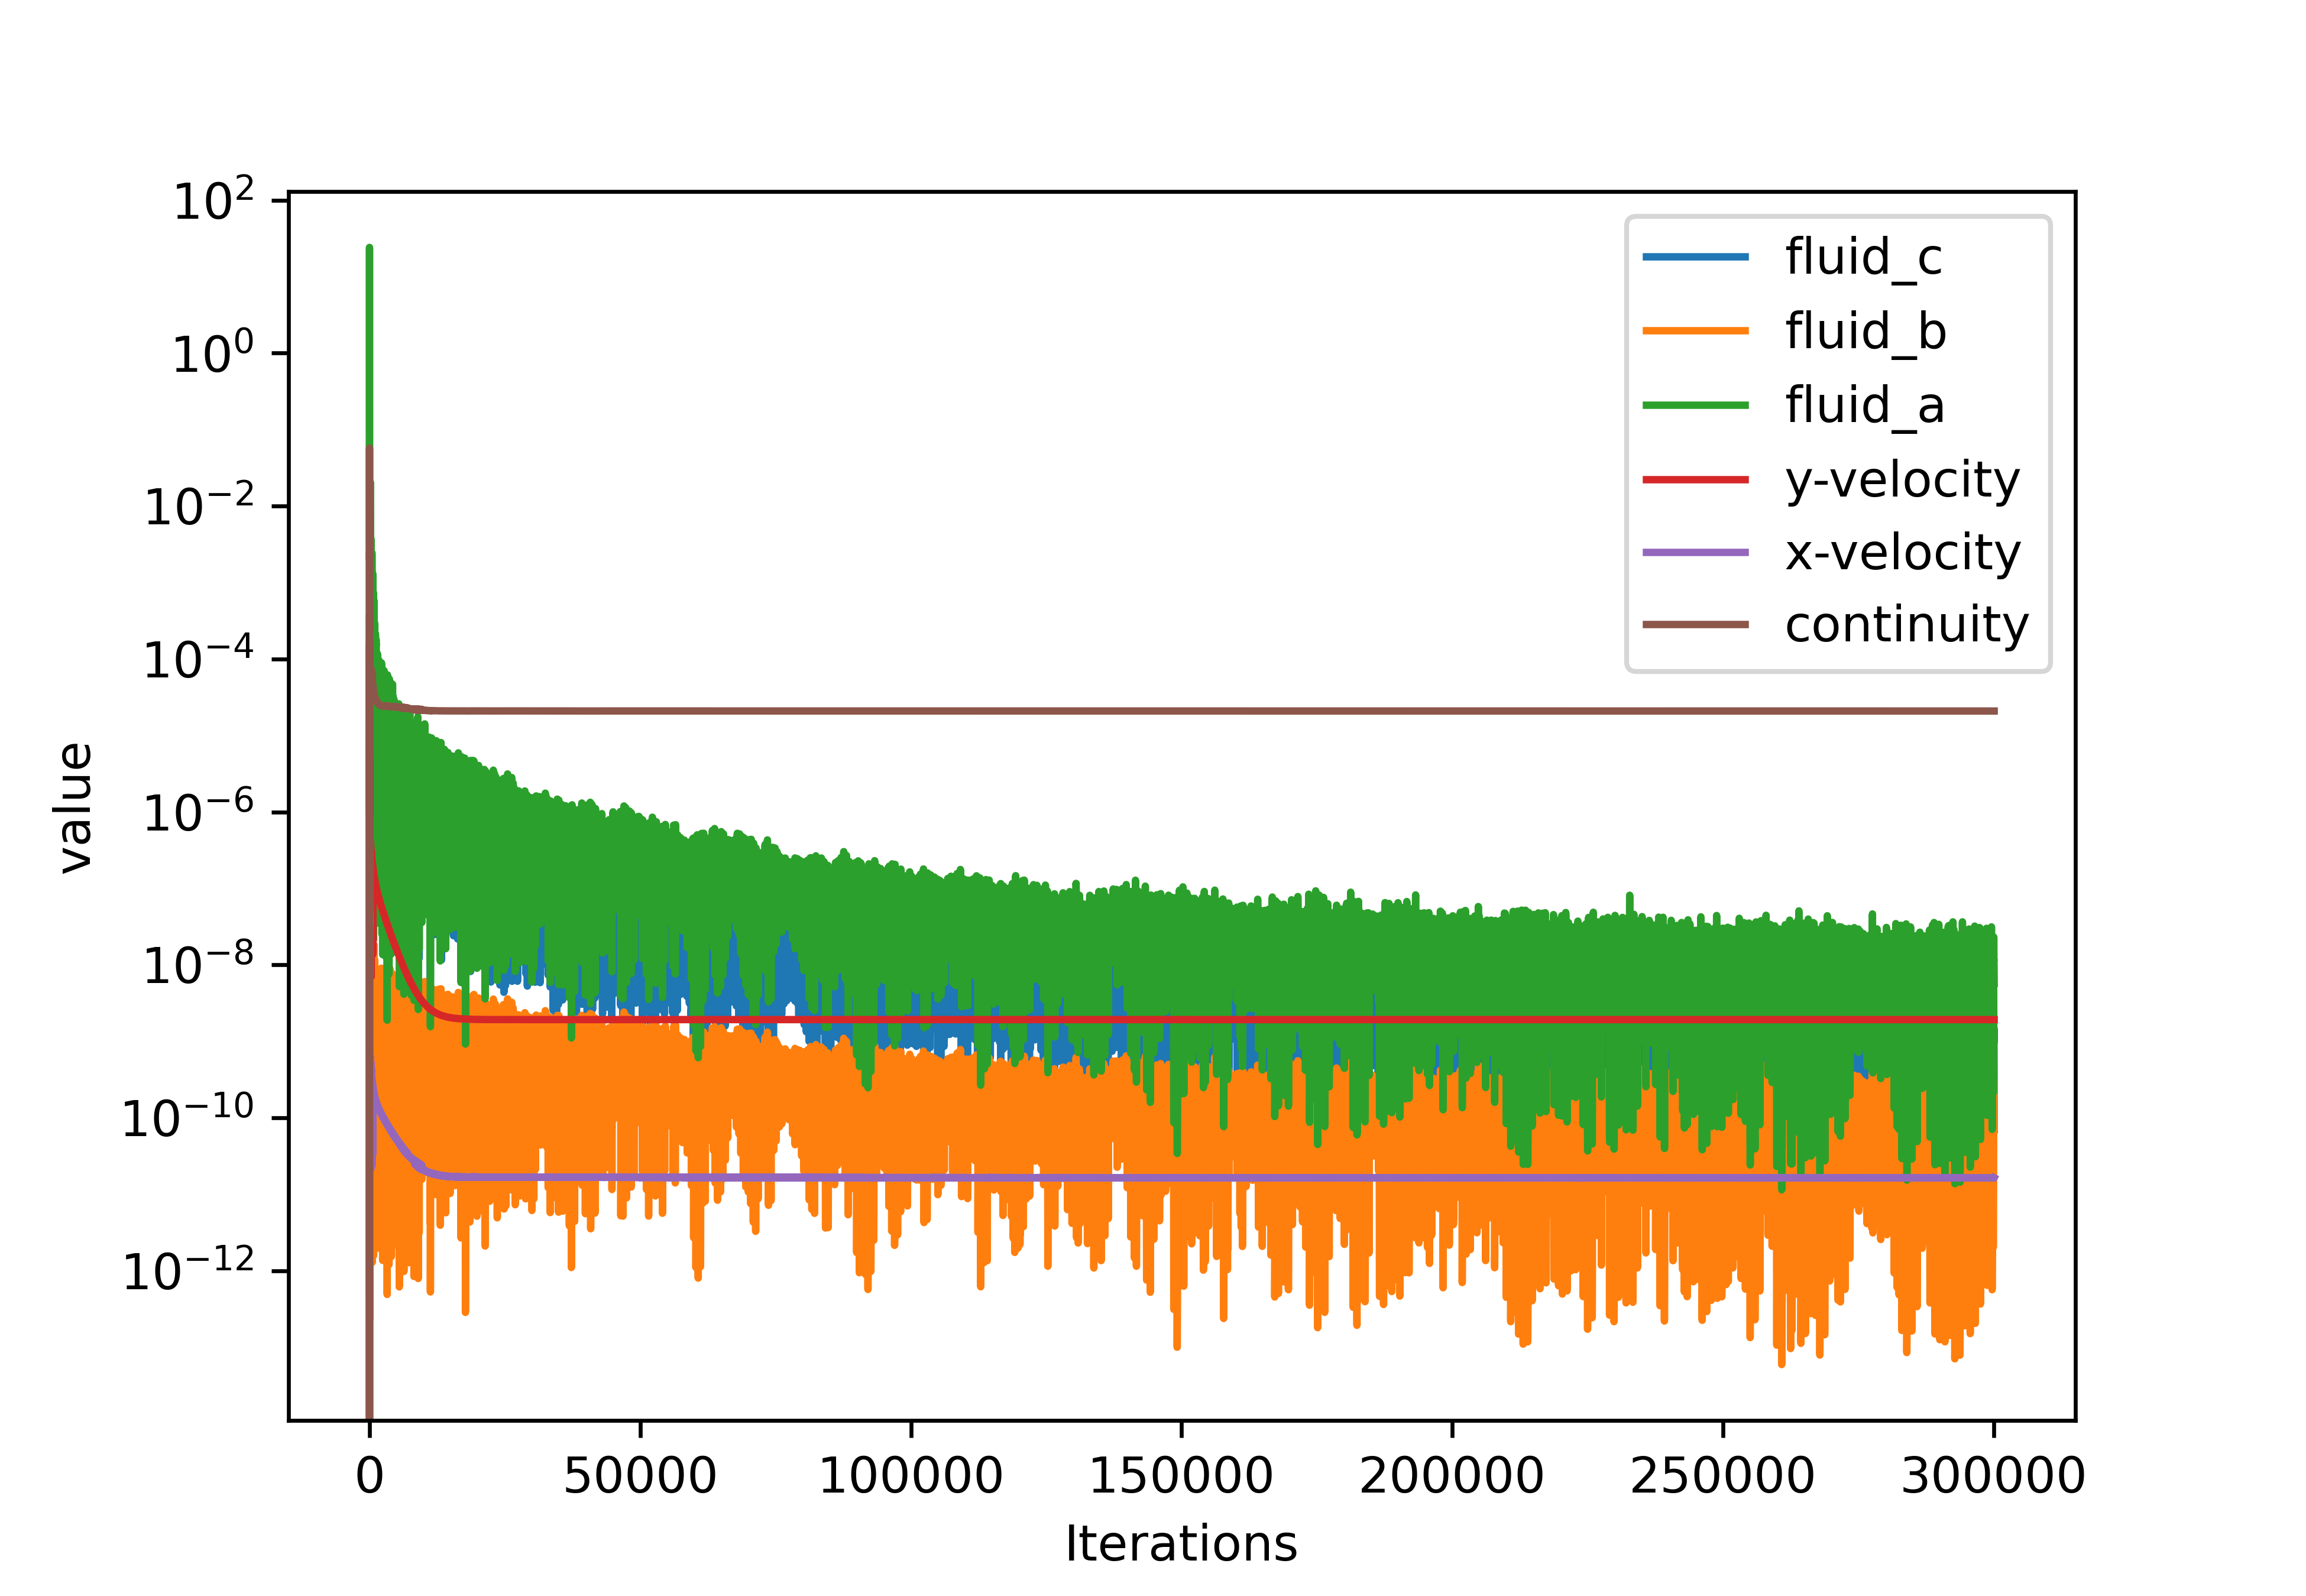
\includegraphics[width=\textwidth]{residuals_h2r3_P500E2_S120E4}
	\caption{example residuals plot}
	\label{fig: residuals}
\end{figure}
To check that the model has converged for a solution step thresholds for the residuals are set. If the residual value for a variable is below the set threshold the solution has converged and the next step is performed. From the plot it can be seen that the residuals do have values of $10^{-5}$ and below so the model performs well for the given example. The values do jump up and down a bit for certain variables that is due to the moving flow and changing fluid composition. For the continuity and velocity variables the residuals are represented by a straight line because once the velocity field is established it does not change any more.

The residuals give an indication on the model's errors and can be used as well to check if the model behaves correctly or which part has to be changed if the solution does not converge or other errors occur.

\section{limitations}
Throughout the model's development process some limitations can be determined which are described in this section.

In it's current state the model can not be run for Peclet-Numbers way higher than the highest investigated which has a value of $2050$. If the Peclet-Number is increased the input velocity goes up as well if the Schmidt-Number is not touched. A higher input velocity needs a lower time step and sometimes a finer mesh to resolve all necessary fluid phenomena happening. Both changes drive up the simulation time exponentially so the amount of computational resources needed for obtaining results in a reasonable amount of time goes way up.

Another limitation is

\chapter{Outlook and Conclusion}
\label{chp:out_con}

\section{Conclusion}

\section{Outlook}

\end{document}